\section{Results}
\label{sec:results}

A general test to develop a sense of Cornerstone's internal bottlenecks is done on a single GPU comparing a case with 100 million using either Hilbert or Morton keys. The test loop contains the code to compute the SFC, do a radix sort, reorder the corresponding particle properties, and update the leaves and then internal tree state; these are the steps needed to compute the octree and have it in a usable state. Immediately we see that the sorting and reordering of particle properties is very dominant in this regime. 

\begin{figure}[h!]
    \centering
    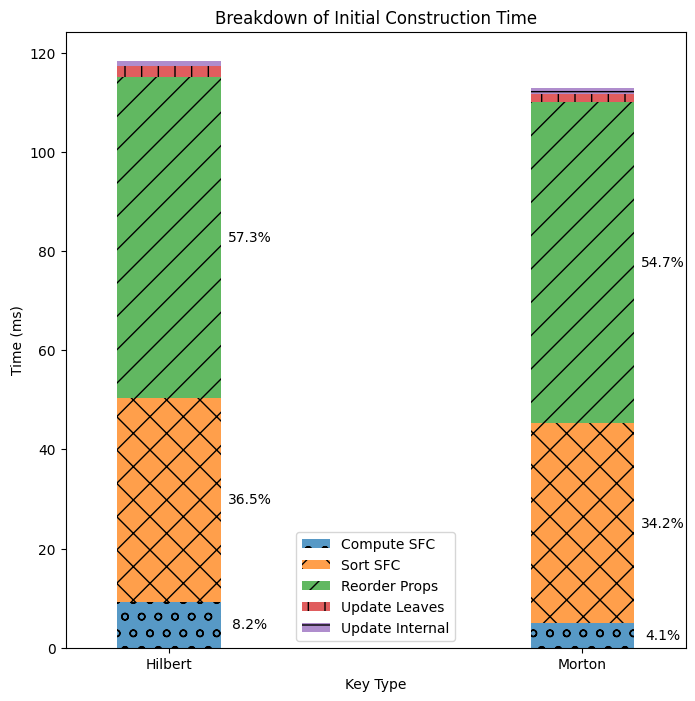
\includegraphics[width=0.45\textwidth]{assets/init_100m.png}
    \caption{Comparison of operations in a broader tree update on a single GPU.}
    \label{fig:keys_100m}
\end{figure}

Figure \ref{fig:keys_100m} breaks down the runtime of both the Hilbert and Morton key cases using the local only build with 100 million particles. The dominant factor in the calculation is the reordering and sorting of the keys and corresponding particles with the actual building of the tree and computation of the space filling curves taking only $\approx 10\%$ of the total build time.

\begin{figure}[h!]
    \centering
    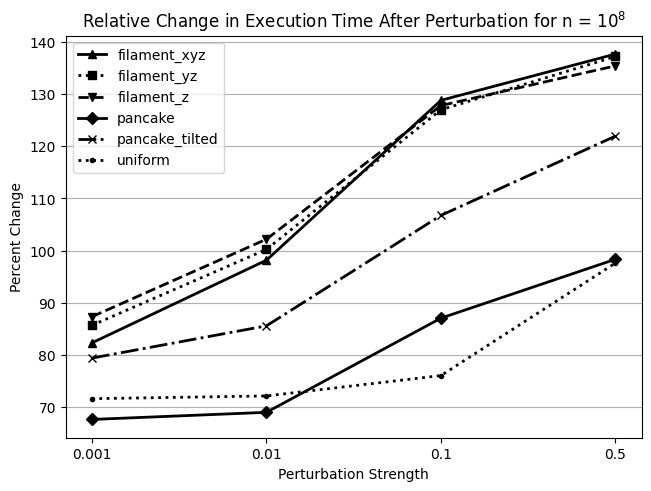
\includegraphics[width=0.45\textwidth]{assets/plotted_n100m.png}
    \caption{Perturbed octree rebalancing time relative to initial build time for different perturbation strengths.}
    \label{fig:plot_100m}
\end{figure}

It is clear that, for the smaller distributions, the perturbations have very little impact on the update time. Only once there are 10 million particles does a clear correlation of perturbation strength to relative update speed become noticeable. At 100 million particles, the effectiveness of the perturbation is even more pronounced.

To establish that perturbations significantly affect the recomputation time of the tree after a perturbation, the recomputation time was measured in relation to the time to initially construct the time as shown in Figure \ref{fig:plot_100m}. The perturbations have varying effectiveness depending on the initial distribution to which they are applied. This is likely due to the fact that the initial distributions are easily expressed by the octree, which applying a perturbation degrades. This is likely why the uniform distribution is not affected greatly by perturbations until a perturbation level of .5, when the filament distributions see a steady performance decrease at increasing perturbation levels. It is important to note that a relative execution time greater than 100\% does not mean updating the octree is slower than reconstructing it from scratch as the perturbed distribution may still take longer to generate from scratch. 

Increasing the perturbation strength often increases the execution time of ReorderXYZ, which was already the most costly part of construction as shown in Figure \ref{fig:breakdown_filament_xyz_100m}. It also mostly eliminates the execution time of UpdateLeaves while leaving the other kernels largely unchanged. As filament\_xyz is the most susceptible to perturbations, it is easiest to notice the changes for that distribution but affects the same kernels in similar ways for different initial distributions.   

Overall in figure \ref{fig:plot_100m} the results were as expected. The general trend shows the rebalancing of the perturbed octree has a dependency on the strength of perturbations. That is as perturbation strength grows time to rebalance grows. What we did not expect to see was that the rebalancing would become significantly greater than even the original build timings, up to $\approx 40\%$ in some cases. This will need to be explored at greater depth in the second half of the project.

\begin{figure}[h!]
    \centering
    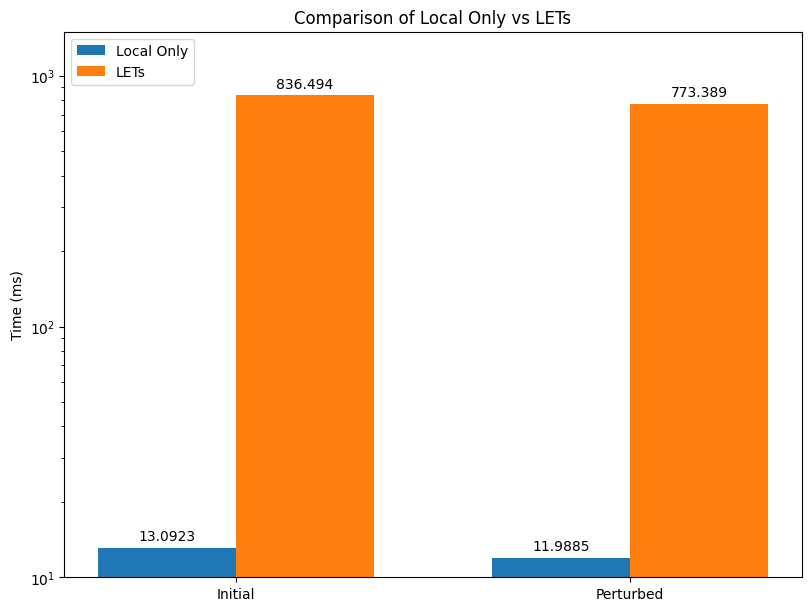
\includegraphics[width=0.45\textwidth]{assets/lets_local_hilbert_10m.png}
    \caption{Comparison of locally essential tree build time vs. local only using 10 million particles, Hilbert keys, and a uniform distribution using 2 ranks, each with their own GPU.}
    \label{fig:plot_lets_local}
\end{figure}

Figure \ref{fig:plot_lets_local} shows the difference in timing in local octree build times vs. the corresponding times for building the distributed domain for the same number of particles. This shows us the overhead of the distributed case over the single node case. Clearly the overhead is significant at approximately two orders of magnitude in this case. On observation of the profile the largest time sync is the calculation of peer ranks according to the multipole acceptance criterion. 
